\section{Experiments}

\subsection{Experimental Setup}
The datasets are split into four categories and the statistics of all datasets are also shown in Table \ref{tab:datasets}. The evaluation metrics for all datasets are shown in Table \ref{tab:dataset_overview_details}, along with more dataset details. For the agents, as described in Section \ref{sub:various_memory_agents}, we consider three categories of agents: \emph{Long-Context Agents}, \emph{RAG agents} and \emph{Agentic Memory Agents}, where \emph{RAG Agents} can be further split into \emph{Simple RAG Agents}, \emph{Embedding-based RAG Agents} and \emph{Structure-Augmented RAG Agents}. We give the detailed introduction of each memory agent in Appendix ~\ref{sec:agents_intro}.  For chunk size settings, we choose a chunk size of 512 for the SH-Doc QA, MH-Doc QA, and LME(S*) tasks in AR, as well as for all tasks in SF. This is mainly because these tasks are composed of long texts synthesized from multiple short texts. For other tasks, we use a chunk size of 4096. Considering computational overhead and API cost, we uniformly use a chunk size of 4096 for Mem0, Cognee, Zep, and MIRIX. We report the detailed settings of the chunk size in Table ~\ref{tab:different_context_length_setting} in Appendix ~\ref{sec:detailed_exp_results}. 
\vspace{-6pt}

% \begin{table*}[t]
%     \centering
%     \setlength{\tabcolsep}{2pt} % default is 6pt
%     \caption{ Overall Performance Comparison. In the absence of a specified model, All RAG agents and commercial memory agents use GPT-4o-mini as the backbone. Thus we highlight the performance of GPT-4o-mini as the reference. SH-QA and MH-QA mean single-hop QA and multi-hop QA. LME(S*) means LongMemEval(S*). FC-SH and FC-MH mean FactConsolidation Single Hop and FactConsolidation Multi Hop, respectively. } 
%     \resizebox{\textwidth}{!}{
%     \begin{tabular}{l|ccccc|ccc|ccc|ccc|c}
%         \rowcolor{headergray}
%         & \multicolumn{5}{c}{\textbf{AR}} & \multicolumn{3}{c}{\textbf{TTL}} & \multicolumn{3}{c}{\textbf{LRU}} & \multicolumn{3}{c}{\textbf{SF}} & Overall \\
%         \rowcolor{headergray}
%         \textbf{Agent Type} & SH-QA & MH-QA & LME(S*) & EventQA & \textbf{Avg.} & MCC & Recom. & \textbf{Avg.} & Summ. & DetQA & \textbf{Avg.} & FC-SH & FC-MH & \textbf{Avg.} & Scores \\
%         \toprule
%         \rowcolor{groupblue}
%         \multicolumn{16}{c}{\emph{Long-Context Agents}} \\
%         GPT-4o            & 72.0 & 51.0 & 32.0 & 77.2 & 58.1 & 87.6 & 12.3 & 50.0 & 32.2 & 77.5 & 54.9 & \textbf{60.0} & \textbf{5.0} & \textbf{32.5} & 48.8  \\
%         GPT-4o-mini       & 64.0 & 43.0 & 30.7 & 59.0 & 49.2 & 82.0 & 15.1 & 48.6 & 28.9 & 63.4 & 46.2  & 45.0 & 5.0 & 25.0 & 42.2  \\
%         GPT-4.1-mini      & 83.0 & \textbf{66.0} & \textbf{55.7} & \textbf{82.6} &    \textbf{71.8} & 75.6 & 16.7 & 46.2 & 41.9 & 56.3 & 49.1 & 36.0 & 5.0 & 20.5 & 46.9 \\
%         Gemini-2.0-Flash  & \textbf{87.0} & 59.0 & 47.0 & 67.2 & 65.1 & 84.0 & 8.7 &  46.4 & 23.9 & 59.2 & 41.6 & 30.0 & 3.0 & 16.5 & 42.4   \\
%         Claude-3.7-Sonnet & 77.0 & 53.0 & 34.0 & 74.6 & 59.7 & \textbf{89.4} & \textbf{18.3} & \textbf{53.9}  & \textbf{52.5} & 71.8 & 62.2 & 43.0 & 2.0 & 22.5 & 49.6 \\
%         \midrule
%         \midrule
%         \rowcolor{headergray}
%         GPT-4o-mini & 64.0 & 43.0 & 30.7 & 59.0 & 49.2 & 82.0 & 15.1 & 48.6 & 28.9 & 63.4 & 46.2 & 45.0 & 5.0 & 25.0 & 42.3 \\
%         \rowcolor{groupgreen}
%         \multicolumn{16}{c}{\emph{Simple RAG Agents}} \\
%         BM25              & 66.0 & 56.0 & 45.3 & \textbf{74.6} & 60.5 & 75.4 & 13.6 & 44.5 & \textbf{19.0} & 52.1 & 35.6 & \underline{48.0} & 3.0 & \underline{25.5} & \underline{41.5}  \\
%         \rowcolor{groupgreen}
%         \multicolumn{16}{c}{\emph{Embedding RAG Agents}} \\
%         Contriever         & 22.0 & 31.0 & 15.7 & 66.8 & 33.9 & 70.6 & 15.2 & 42.9 & 17.2 & 42.3 & 29.8 & 18.0 & \textbf{7.0} &  12.5 & 29.8 \\
%         Text-Embed-3-Small & 60.0 & 44.0 & 48.3 & 63.0 & 53.8 & 70.0 & \underline{15.3} & 42.7 & 17.7 & 54.9 & 36.3 & 28.0 & 3.0 & 15.5 & 37.1  \\
%         Text-Embed-3-Large & 54.0 & 44.0 & 50.3 & 70.0 & 54.6 & 72.4 & \textbf{16.2} & 44.3 & 18.2 & 56.3 & \underline{37.3} & 28.0 & 4.0 & 16.0 & 38.0 \\
%         Qwen3-Embedding-4B & 57.0 & 47.0 & 43.3 & \underline{71.4} & 54.7 & \textbf{78.0} & 12.2 & \textbf{45.1} & 14.8 & \underline{59.2} & 37.0 & 29.0 & 3.0 & 16.0 & 38.2 \\

%         \rowcolor{groupgreen}
%         \multicolumn{16}{c}{\emph{Structure-Augmented RAG Agents}} \\
%         RAPTOR      & 29.0 & 38.0 & 34.3 & 45.8 & 36.8 & 59.4 & 12.3 & 35.9 & 13.4 & 42.3 & 27.9 & 14.0 & 1.0 & 7.5 & 27.0 \\
%         GraphRAG    & 47.0 & 47.0 & 35.0 & 34.4 & 40.9 & 39.8 & 9.8 & 24.8 & 0.4 & 39.4 & 19.9 & 14.0 & 2.0 & 8.0 & 23.4 \\
%         MemoRAG     & 29.0 & 33.0 & 20.0 & 56.0 & 34.5 & \underline{77.0} & 13.1 & \textbf{45.1} & 9.2 & 50.7 & 30.0 & 21.0 & \textbf{7.0} & 14.0 & 30.9 \\
%         HippoRAG-v2 & \textbf{76.0} & \underline{66.0} & \underline{50.7} & 67.6 & \textbf{65.1} & 61.4 & 10.2 & 35.8  & 14.6 & 57.7 & 36.2 & \textbf{54.0} & 5.0 & \textbf{29.5} & \textbf{41.6} \\
%         Mem0        & 25.0 & 32.0 & 36.0 & 37.5 & 32.6 & 32.4 & 10.0 & 21.2 & 4.8 & 36.6 & 20.7 & 18.0 & 2.0 & 10.0 & 21.1 \\
%         Cognee      & 31.0 & 26.0 & 29.3 & 26.8 & 28.3 & 35.4 & 10.1 & 22.8 & 2.3 & 29.6 & 16.0 & 28.0 & 3.0 & 15.5 & 20.6 \\
%         Zep            & 44.0 & 25.0 & 38.3 & 42.5 & 37.5 & 62.8 & 12.1 & 37.5 & 4.2 & 28.2 & 16.2 & 7.0 & 3.0 & 5.0 & 24.0 \\
%         \rowcolor{grouppink}
%         \multicolumn{16}{c}{\emph{Agentic Memory Agents}} \\
%         Self-RAG       & 35.0 & 42.0 & 25.7 & 31.8 & 33.6 & 11.6 & 12.8 & 12.2 & 0.9 & 35.2 & 18.1 & 19.0 & 3.0 & 11.0 & 18.7 \\
%         MemGPT         & 41.0 & 38.0 & 32.0 & 26.2 & 34.3 & 67.6 & 14.0 & 40.8 & 2.5 &  42.3 & 22.4 & 28.0 & 3.0 & 15.5 & 28.3 \\
%         MIRIX           & 62.0 & 61.0 & 37.3 & 29.8 & 47.5 & 38.4 & 9.8 & 24.1 & 9.9 & 40.8 & 25.4 & 14.0 & 2.0 & 8.0  & 26.2 \\
%         MIRIX (4.1-mini)  & \underline{73.0} & \textbf{75.0} & \textbf{51.0} & 53.0 & \underline{63.0} & 61.0 & 10.3 &  35.7 & \underline{18.9} & \textbf{62.0} & \textbf{40.5} & 20.0 & 3.0 & 11.5 & 37.7 \\
%         \bottomrule
%     \end{tabular}
%     }
%     \vspace{-8pt}
% \label{tab:overall_performance_comparison}
% \end{table*}




\begin{table*}[t]
    \centering
    \setlength{\tabcolsep}{2pt} % default is 6pt
    \caption{Overall Performance Comparison. In the absence of a specified model, All RAG agents and commercial memory agents use GPT-4o-mini as the backbone. Thus we highlight the performance of GPT-4o-mini as the reference. FC-SH and FC-MH mean FactConsolidation Single Hop and FactConsolidation Multi Hop, respectively. Best viewed in colors.} 
    \resizebox{\textwidth}{!}{
    \begin{tabular}{l|cccc>{\columncolor{avgcolor}}c|cc>{\columncolor{avgcolor}}c|cc>{\columncolor{avgcolor}}c|cc>{\columncolor{avgcolor}}c|>{\columncolor{overallcolor}}c}
        \rowcolor{headergray}
        & \multicolumn{5}{c}{\textbf{AR}} & \multicolumn{3}{c}{\textbf{TTL}} & \multicolumn{3}{c}{\textbf{LRU}} & \multicolumn{3}{c}{\textbf{SF}} & \cellcolor{overallcolor}Overall \\
        \rowcolor{headergray}
        \textbf{Agent Type} & SH-QA & MH-QA & LME(S*) & EventQA & \cellcolor{avgcolor}\textbf{Avg.} & MCC & Recom. & \cellcolor{avgcolor}\textbf{Avg.} & Summ. & DetQA & \cellcolor{avgcolor}\textbf{Avg.} & FC-SH & FC-MH & \cellcolor{avgcolor}\textbf{Avg.} & \cellcolor{overallcolor}Scores \\
        \toprule
        \rowcolor{groupblue}
        \multicolumn{16}{c}{\emph{Long-Context Agents}} \\
        GPT-4o (128K)           & 72.0 & 51.0 & 32.0 & 77.2 & 58.1 & 87.6 & 12.3 & 50.0 & 32.2 & 77.5 & 54.9 & 60.0 & 5.0 & 32.5 & 48.8  \\
        GPT-4o-mini (128K)      & 64.0 & 43.0 & 30.7 & 59.0 & 49.2 & 82.0 & 15.1 & 48.6 & 28.9 & 63.4 & 46.2  & 45.0 & 5.0 & 25.0 & 42.2  \\
        
        Claude-3.7-Sonnet (200K) & 77.0 & 53.0 & 34.0 & 74.6 & 59.7 & \textbf{89.4} & \textbf{18.3} & \textbf{53.9}  & 52.5 & 71.8 & 62.2 & 43.0 & 2.0 & 22.5 & 49.6 \\
        
        GPT-5-mini (400K) & 85.0 & \textbf{71.0} & \textbf{63.3} & \textbf{78.2} & \textbf{74.4} & 84.0 & 13.2 & 48.6 & \textbf{56.3} & \textbf{76.1} & \textbf{66.2} & 78.0 & 28.0 & \textbf{53.0} & \textbf{60.6} \\

        GPT-4.1-mini (1M)     & 83.0 & 66.0 & 55.7 & 82.6 & 71.8 & 75.6 & 16.7 & 46.2 & 41.9 & 56.3 & 49.1 & 36.0 & 5.0 & 20.5 & 46.9 \\


        Gemini-2.0-Flash (1M)  & \textbf{87.0} & 59.0 & 47.0 & 67.2 & 65.1 & 84.0 & 8.7 & 46.4 & 23.9 & 59.2 & 41.6 & 30.0 & 3.0 & 16.5 & 42.4   \\


        % GPT-5-mini \\
        \midrule
        \midrule
        \rowcolor{headergray}
        GPT-4o-mini & 64.0 & 43.0 & 30.7 & 59.0 & \cellcolor{avgcolor}49.2 & 82.0 & 15.1 & \cellcolor{avgcolor}48.6 & 28.9 & 63.4 & \cellcolor{avgcolor}46.2 & 45.0 & 5.0 & \cellcolor{avgcolor}25.0 & \cellcolor{overallcolor}42.3 \\
        \rowcolor{groupgreen}
        \multicolumn{16}{c}{\emph{Simple RAG Agents}} \\
        BM25              & 66.0 & 56.0 & 45.3 & \textbf{74.6} & 60.5 & 75.4 & 13.6 & 44.5 & \textbf{19.0} & 52.1 & 35.6 & \underline{48.0} & 3.0 & \underline{25.5} & \underline{41.5}  \\
        \rowcolor{groupgreen}
        \multicolumn{16}{c}{\emph{Embedding RAG Agents}} \\
        Contriever         & 22.0 & 31.0 & 15.7 & 66.8 & 33.9 & 70.6 & 15.2 & 42.9 & 17.2 & 42.3 & 29.8 & 18.0 & \textbf{7.0} & 12.5 & 29.8 \\
        Text-Embed-3-Small & 60.0 & 44.0 & 48.3 & 63.0 & 53.8 & 70.0 & \underline{15.3} & 42.7 & 17.7 & 54.9 & 36.3 & 28.0 & 3.0 & 15.5 & 37.1  \\
        Text-Embed-3-Large & 54.0 & 44.0 & 50.3 & 70.0 & 54.6 & 72.4 & \textbf{16.2} & 44.3 & 18.2 & 56.3 & \underline{37.3} & 28.0 & 4.0 & 16.0 & 38.0 \\
        Qwen3-Embedding-4B & 57.0 & 47.0 & 43.3 & \underline{71.4} & 54.7 & \textbf{78.0} & 12.2 & \textbf{45.1} & 14.8 & \underline{59.2} & 37.0 & 29.0 & 3.0 & 16.0 & 38.2 \\

        \rowcolor{groupgreen}
        \multicolumn{16}{c}{\emph{Structure-Augmented RAG Agents}} \\
        RAPTOR      & 29.0 & 38.0 & 34.3 & 45.8 & 36.8 & 59.4 & 12.3 & 35.9 & 13.4 & 42.3 & 27.9 & 14.0 & 1.0 & 7.5 & 27.0 \\
        GraphRAG    & 47.0 & 47.0 & 35.0 & 34.4 & 40.9 & 39.8 & 9.8 & 24.8 & 0.4 & 39.4 & 19.9 & 14.0 & 2.0 & 8.0 & 23.4 \\
        MemoRAG     & 29.0 & 33.0 & 20.0 & 56.0 & 34.5 & \underline{77.0} & 13.1 & \textbf{45.1} & 9.2 & 50.7 & 30.0 & 21.0 & \textbf{7.0} & 14.0 & 30.9 \\
        HippoRAG-v2 & \textbf{76.0} & \underline{66.0} & \underline{50.7} & 67.6 & \textbf{65.1} & 61.4 & 10.2 & 35.8  & 14.6 & 57.7 & 36.2 & \textbf{54.0} & 5.0 & \textbf{29.5} & \textbf{41.6} \\
        Mem0        & 25.0 & 32.0 & 36.0 & 37.5 & 32.6 & 32.4 & 10.0 & 21.2 & 4.8 & 36.6 & 20.7 & 18.0 & 2.0 & 10.0 & 21.1 \\
        Cognee      & 31.0 & 26.0 & 29.3 & 26.8 & 28.3 & 35.4 & 10.1 & 22.8 & 2.3 & 29.6 & 16.0 & 28.0 & 3.0 & 15.5 & 20.6 \\
        Zep            & 44.0 & 25.0 & 38.3 & 42.5 & 37.5 & 62.8 & 12.1 & 37.5 & 4.2 & 28.2 & 16.2 & 7.0 & 3.0 & 5.0 & 24.0 \\
        \rowcolor{grouppink}
        \multicolumn{16}{c}{\emph{Agentic Memory Agents}} \\
        Self-RAG       & 35.0 & 42.0 & 25.7 & 31.8 & 33.6 & 11.6 & 12.8 & 12.2 & 0.9 & 35.2 & 18.1 & 19.0 & 3.0 & 11.0 & 18.7 \\
        MemGPT         & 41.0 & 38.0 & 32.0 & 26.2 & 34.3 & 67.6 & 14.0 & 40.8 & 2.5 & 42.3 & 22.4 & 28.0 & 3.0 & 15.5 & 28.3 \\
        MIRIX           & 62.0 & 61.0 & 37.3 & 29.8 & 47.5 & 38.4 & 9.8 & 24.1 & 9.9 & 40.8 & 25.4 & 14.0 & 2.0 & 8.0 & 26.2 \\
        MIRIX (4.1-mini)  & \underline{73.0} & \textbf{75.0} & \textbf{51.0} & 53.0 & \underline{63.0} & 61.0 & 10.3 & 35.7 & \underline{18.9} & \textbf{62.0} & \textbf{40.5} & 20.0 & 3.0 & 11.5 & 37.7 \\
        \bottomrule
    \end{tabular}
    }
    \vspace{-8pt}
\label{tab:overall_performance_comparison}
\end{table*}


\subsection{Overall Performance Comparison}
Table~\ref{tab:overall_performance_comparison} presents the overall performance across different benchmarks. We summarize the key findings as follows: \textbf{(1) Superiority of RAG methods in Accurate Retrieval Tasks.} Most RAG Agents are better than the backbone model ``GPT-4o-mini'' in the tasks within the Accurate Retrieval Category. This matches our intuition where RAG agents typically excel at extracting a small snippet of text that is crucial for answering the question. \textbf{(2) Superiority of Long-Context Models in Test-Time Learning and Long-Range Understanding.} Long-context models achieve the best performance on TTL and LRU. This highlights a fundamental limitation of RAG methods and commercial memory agents, which still follow an agentic RAG paradigm. These systems retrieve only partial information from the past context, lacking the ability to capture a holistic understanding of the input—let alone perform learning across it. \textbf{(3) Limitation of All Existing Methods on Selective Forgetting.} Although being a well-discussed task in model-editing community~\citep{SERAC,alphaedit}, forgetting out-of-date memory poses a significant challenge on memory agents. We observe that all methods fail on the multi-hop situation (with achieving at most 28\% accuracy). Only long context agents can achieve fairly reasonable results on single-hop scenarios. In Section \ref{sec:factcon_validation}, we show that current reasoning models can have much better performance, while it does not change the conclusion that Selective Forgetting still poses a significant challenge to all memory mechanisms. 



\subsection{Analysis and Ablation Study}

In this section, we present experiments and analysis along five dimensions: input chunk size, retrieval top-$k$, backbone model, and dataset validation. Additional results are provided in the appendix, including compuational latency (Appendix \ref{sub:latency_analysis}), context length analysis (Appendix \ref{sub:different_context_length}), latency and GPU memory usage comparisons (Appendix \ref{sub:latency_analysis}, \ref{sub:gpu_memory_usage_comparison}),  further details on chunk size and top-$k$ ablations (Appendix \ref{sub:input_chunk_ablation}, \ref{sub:results_on_topk}), as well as the Cost-Performance estimation (Appendix \ref{app:cost_performance}).



\subsubsection{Ablation Study on Input Chunk Size}

To understand how chunk size impacts performance, particularly for RAG methods and agentic memory agents, we conduct an additional analysis where we vary the chunk size while fixing the number of retrieved chunks to 10. 
The results are presented in Figure~\ref{fig:ruler_chunk_size}.
From the figure, we observe %the following:(1) In the SH-Doc QA task, reducing chunk size has little effect on BM25 performance. This is expected, as BM25 relies on term-frequency-based scoring and document-level ranking, and does not inherently benefit from finer-grained segmentation beyond the impact on term distributions. In contrast, embedding-based methods—including MemGPT, which uses \texttt{text-embedding-3-small} as its retriever—consistently perform better with smaller chunks. This suggests that finer segmentation improves the granularity and relevance of retrieved results for models that rely on dense semantic representations.(2) In $\infty$Bench-Sum, however, smaller chunk sizes lead to worse performance. This task requires the agent to summarize an entire conversation, and smaller chunks correspond to fewer available tokens per retrieval. As a result, the agent has access to less context, which degrades summarization quality.The results suggest  
that when resources permit, using smaller chunk sizes and increasing the number of retrieval calls during memory construction can improve performance on Accurate Retrieval (AR) tasks. Finer-grained segmentation enhances the relevance of retrieved information, particularly for embedding-based methods. However, for tasks requiring Long-Range Understanding (LRU), varying the chunk size hurts the performance. This is likely because RAG methods are inherently less suited for tasks that demand integration of information across a large, coherent context.

\begin{figure}[t]
    \centering
    \begin{subfigure}[b]{0.495\linewidth}
        \centering
        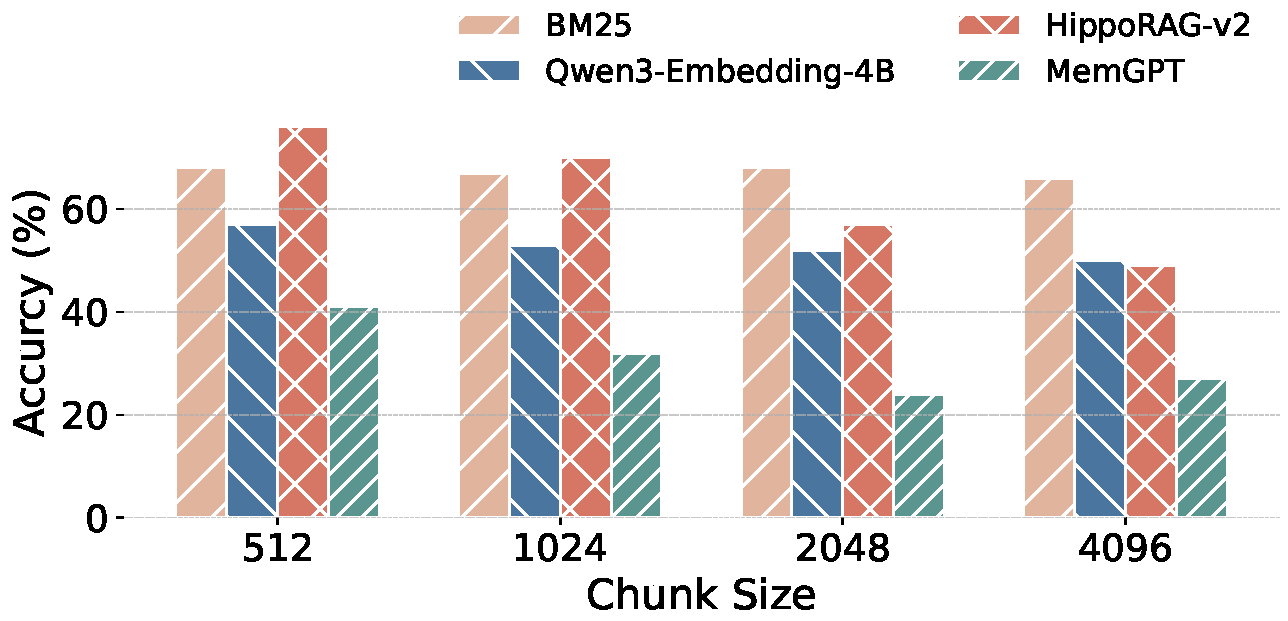
\includegraphics[width=\linewidth]{figures/ruler_chunk_size.pdf}
        \caption{SH-Doc QA performance}
        \label{fig:ruler_chunk}
    \end{subfigure}
    \hfill
    \begin{subfigure}[b]{0.495\linewidth}
        \centering
        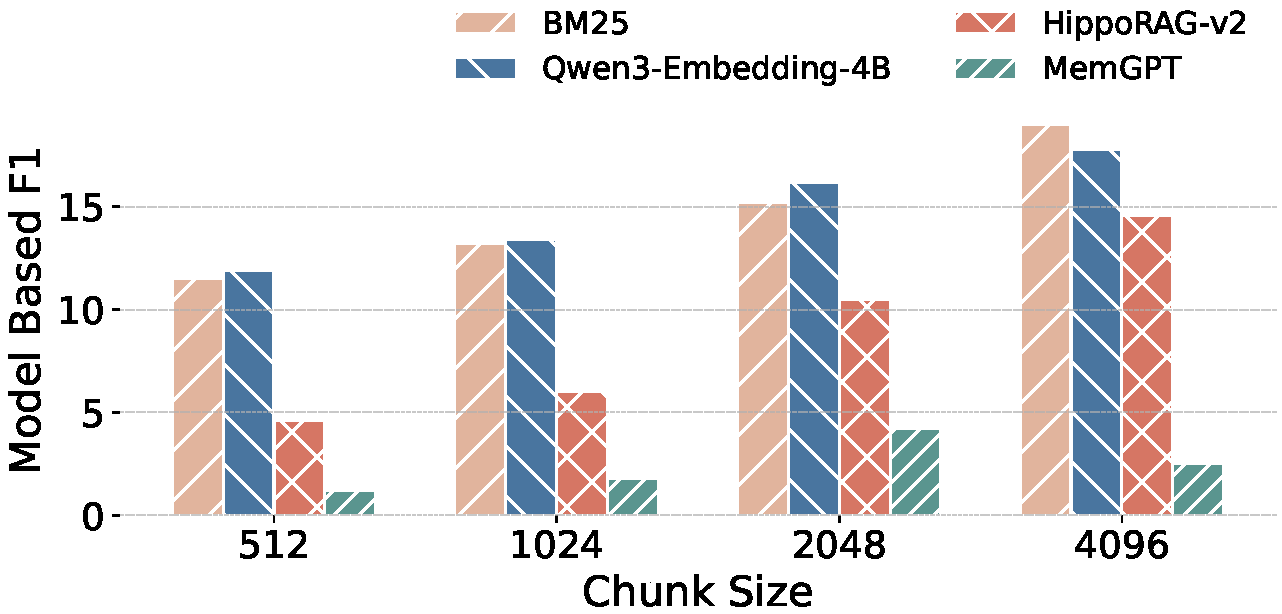
\includegraphics[width=\linewidth]{figures/infty_sum_chunk_size.pdf}
        \caption{$\infty$Bench-Sum performance}
        \label{fig:infinite_sum_chunk}
    \end{subfigure}
    \caption{Performances on SH-Doc QA and $\infty$-Bench-Sum with different chunk sizes.}
    \label{fig:ruler_chunk_size}
    \vspace{-10pt}
\end{figure}





\subsubsection{Ablation Study on Retrieval TopK}
In our experiments, although we report most results with the number of retrieved chunks set to 10 in Table~\ref{tab:overall_performance_comparison}, we also conducted ablation studies with varying retrieval sizes. A subset of these results is visualized in Figure~\ref{fig:retrieve_topk_ablation}, with the full results provided in Table~\ref{tab:retrieval_topk_ablation} in Appendix ~\ref{sec:detailed_exp_results}.
The results indicate that increasing the number of retrieved chunks generally improves performance across most tasks. It is worth noting that, with a chunk size of 4096 tokens, retrieving 10 chunks already yields an input of approximately 40k tokens. This places significant demands on model capacity. Due to this high token volume, we do not evaluate settings with 20 retrieved chunks. 



\begin{figure}
\centering
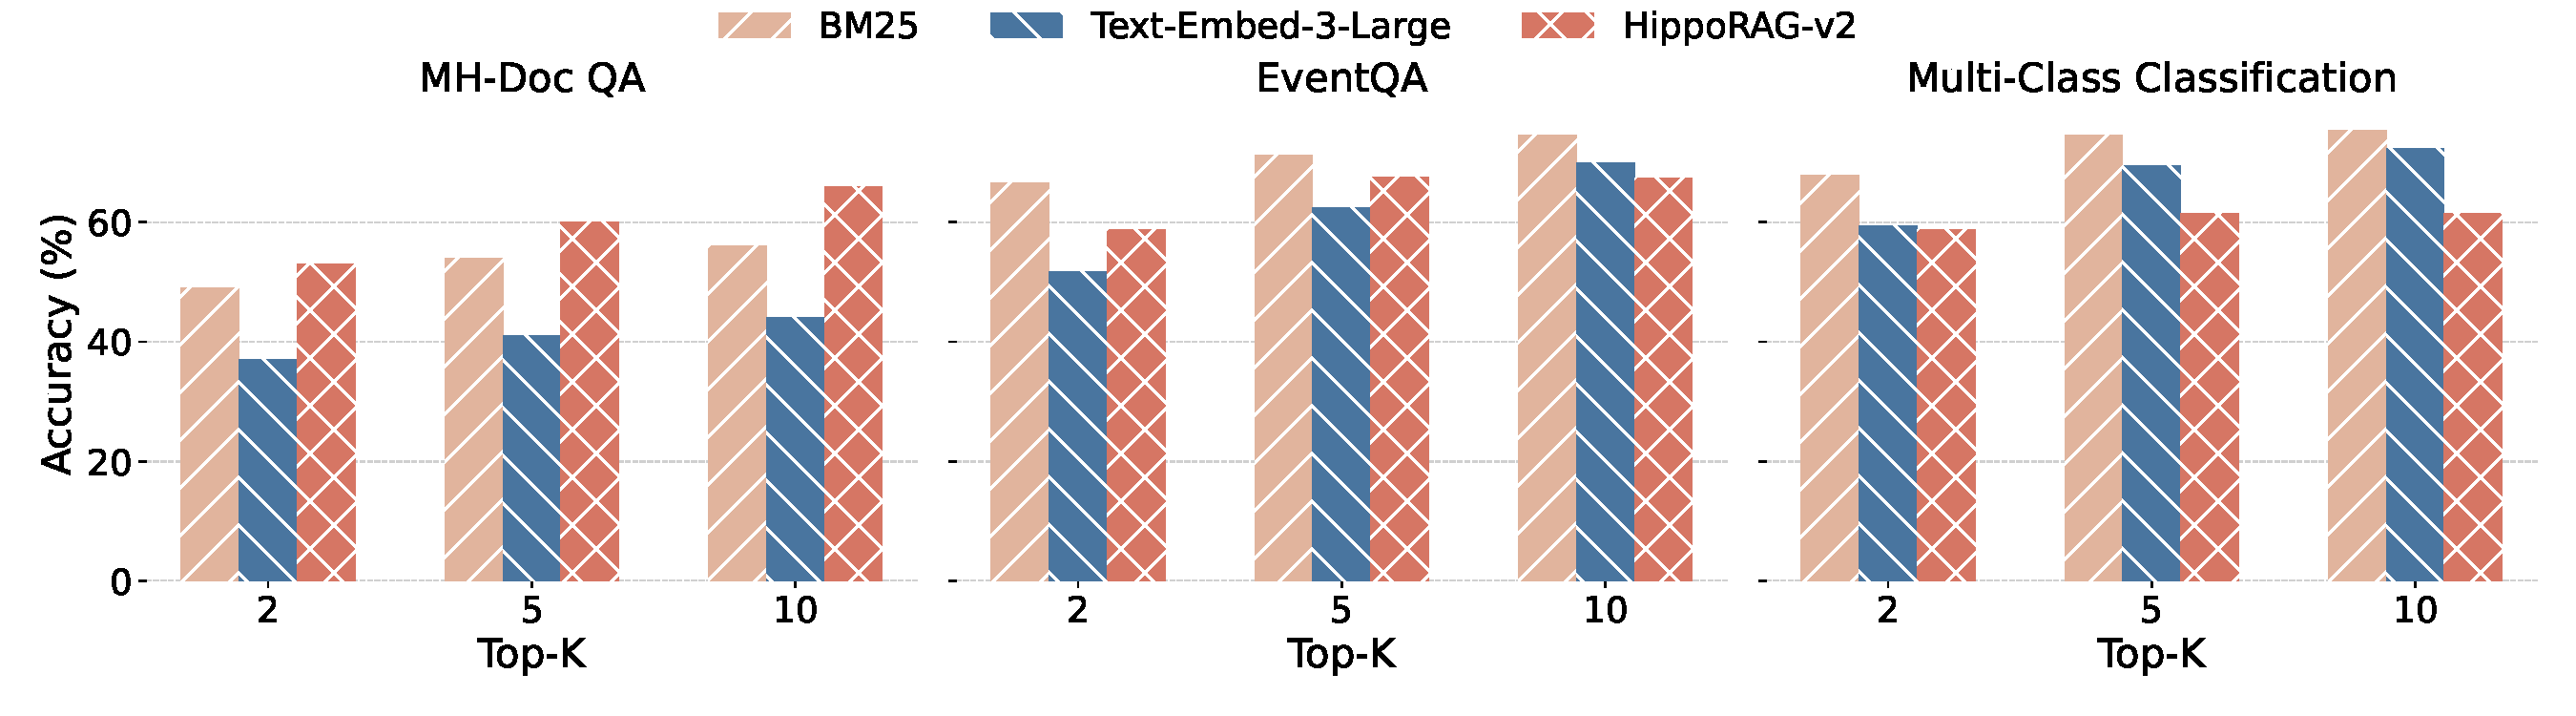
\includegraphics[width=\linewidth]{figures/retrieve_ablation.pdf}
\caption{The accuracies on different benchmarks when varying the retrieval top-k to be 2, 5 and 10.}
\label{fig:retrieve_topk_ablation}
\vspace{-10pt}
\end{figure}


\subsubsection{Ablation Study on Backbone Model}

To investigate how different backbone models impact the performance of various memory agents, we experimented with three different backbone models and selected four representative methods from both the RAG Agents and Agentic Memory categories. The complete experimental results are presented in Table ~\ref{tab:different_backbone}. Our findings show that for RAG Agents, once the backbone is sufficiently strong, it no longer serves as the main performance bottleneck. Compared to the default setup, upgrading to a more powerful model like GPT-4.1-mini yields only marginal improvements. In contrast, the main results in Table ~\ref{tab:overall_performance_comparison} for the MIRIX method under the Agentic Memory category, using a stronger backbone leads to substantial performance gains. This suggests that future advances in backbone models could further boost the effectiveness of Agentic Memory methods.

\begin{table*}
    \centering
    \caption{Performance comparison on three different backbone LLMs and four representative memory agents. We choose one dataset from every competency to evaluate agent performance. }
    \resizebox{\textwidth}{!}{
    \begin{tabular}{cc|ccccc}
        \toprule
          \rowcolor{headergray}
          \textbf{Agent Type} & Backbone Model  & EventQA & Recom & $\infty$Bench-Sum & FactCon-SH & Avg. \\
          \midrule
            & GPT-4o-mini      & 74.6 & 13.6 & 19.0 & 48.0 & 38.8  \\
          BM25  & GPT-4.1-mini     & 76.4 & 14.0 & 19.4 & 51.0 & 40.2  \\
            & Gemini-2.0-Flash & 70.8 & 10.0 & 18.9 & 47.0 & 36.7 \\
          \midrule
            & GPT-4o-mini       & 63.0 & 15.3 & 17.7 & 28.0  & 31.0 \\
          Text-Embed-3-Small & GPT-4.1-mini      & 62.0 & 15.5 & 17.9 & 30.0 & 31.4  \\
            & Gemini-2.0-Flash  & 64.0 & 10.3 & 17.2 & 27.0 & 29.6 \\
          \midrule
            & GPT-4o-mini        & 34.4 & 9.8 & 0.4 & 14.0 & 14.7   \\
          GraphRAG & GPT-4.1-mini        & 39.0 & 10.3 & 1.2 & 16.0 & 16.6   \\
            & Gemini-2.0-Flash     & 36.2 & 7.2 & 0.8 & 13.0 & 14.3   \\
          \midrule
          \multirow{2}{*}{MIRIX}  & GPT-4o-mini  & 29.8 & 9.8 & 9.9 & 14.0 & 15.9  \\
          & GPT-4.1-mini  & 53.0 \textbf{(23.2$\uparrow$)} & 10.3 \textbf{(0.5$\uparrow$)} & 18.9 \textbf{(9.0$\uparrow$)} & 20.0 \textbf{(6.0$\uparrow$)} & 25.6 \textbf{(9.7$\uparrow$)}   \\
          \bottomrule
        \end{tabular}}
    \label{tab:different_backbone}
     \centering
     
\end{table*}


\subsubsection{Validation of Dataset FactConsolidation}
\label{sec:factcon_validation}

\begin{wraptable}{r}{0.48\textwidth} 
    \centering
    \vspace{-12pt}
    \caption{Performances of reasoning models on the dataset FactConsolidation.}
      \resizebox{0.4\textwidth}{!}{
    \begin{tabular}{c|cc|cc}
        \toprule
          & \multicolumn{2}{c|}{FactCon-SH} & \multicolumn{2}{c}{FactCon-MH} \\
         & 6K & 32K & 6K & 32K \\
        \midrule
        GPT-4o   & 92.0 & 88.0 & 28.0 & 10.0 \\
        O4-mini  & \textbf{100.0} & 61.0 & \textbf{80.0} & 14.0 \\
        \bottomrule
    \end{tabular}
    }
\label{tab:factconsolidation_check}
\vspace{-10pt}
\end{wraptable}

As the performance of different models on this dataset
remains drastically low, we turn to the stronger reasoning model o4-mini and validate our dataset by checking the performance of o4-mini on a smaller version
of this dataset. The results are shown in Table ~\ref{tab:factconsolidation_check}.  We found that on the 6K version of the FactCon-SH dataset, both models perform well and are generally able to complete the task effectively. However, their performance drops when the context length increases to 32K. Similarly, on the 6K version of the FactCon-MH dataset, the stronger O4-mini reasoning model achieves a decent score of 80.0, but its performance significantly drops to 14.0 when the context window reaches 32K. This indicates that our dataset is solvable under short-context settings, but current memory agents still lack strong long-range reasoning capabilities, making them unable to handle the task when presented with longer historical inputs.

% {
% \color{blue}\subsubsection{API Cost and Token Usage}
% }
